% ============================================================================
% CTW-VA-2026: Vendor-Specific Refusal Patterns in LLM Responses to
% Taiwan-Political Prompts
%
% Compile with XeLaTeX (for xeCJK Chinese support):
%   xelatex main && biber main && xelatex main && xelatex main
%
% Or use `make` (see Makefile).
% ============================================================================
\documentclass[11pt,letterpaper]{article}

% ── Layout ───────────────────────────────────────────────────────────────
\usepackage[margin=1in]{geometry}
\usepackage{parskip}           % blank line between paragraphs, no indent
\usepackage{microtype}
\setlength{\emergencystretch}{3em}

% ── Fonts + CJK ──────────────────────────────────────────────────────────
\usepackage{fontspec}
\usepackage{xeCJK}
% Fall back to system fonts if these aren't present (user can override)
\IfFontExistsTF{Helvetica Neue}{\setmainfont{Helvetica Neue}}{}
\IfFontExistsTF{PingFang TC}{\setCJKmainfont{PingFang TC}}{%
  \IfFontExistsTF{Noto Sans CJK TC}{\setCJKmainfont{Noto Sans CJK TC}}{}}

% ── Math / tables / figures ──────────────────────────────────────────────
\usepackage{amsmath,amssymb}
\usepackage{booktabs}
\usepackage{array}
\usepackage{graphicx}
\graphicspath{{../paper_figures/}}
\usepackage{caption}
\captionsetup{font=small,labelfont=bf,skip=6pt}
\usepackage{subcaption}

% ── Colors + links ───────────────────────────────────────────────────────
\usepackage[dvipsnames]{xcolor}
\usepackage[colorlinks=true,
            linkcolor=black,
            citecolor=Sepia,
            urlcolor=NavyBlue]{hyperref}

% ── Bibliography ─────────────────────────────────────────────────────────
\usepackage[backend=biber,style=authoryear,natbib=true,maxcitenames=2,
            sorting=nyt]{biblatex}
\addbibresource{refs.bib}

% ── Code / verbatim ──────────────────────────────────────────────────────
\usepackage{xurl}

% ── Custom macros ────────────────────────────────────────────────────────
\newcommand{\vendor}[1]{\textsf{#1}}
\newcommand{\todo}[1]{\textcolor{red}{\textbf{[TODO: #1]}}}
\newcommand{\ci}[2]{[#1,\,#2]}
\newcommand{\pp}{\,\text{pp}}

% ── Title ────────────────────────────────────────────────────────────────
\title{Vendor-Specific Refusal Patterns in LLM Responses to\\
       Taiwan-Political Prompts: Evidence Against a Monolithic\\
       East--West Alignment Dichotomy}
\author{Ch Tseng\thanks{Independent researcher. Correspondence:
        \href{mailto:chtseng.neural@gmail.com}{chtseng.neural@gmail.com}.
        Code, data, and labeling protocol available at
        \url{https://github.com/chtseng-neural/Civatas-TW}.}}
\date{\today}


\begin{document}

\maketitle

\begin{abstract}
\todo{Write last. Key points:
(i) audit of 5 LLM vendors on 200 Taiwan-political prompts × 5 = 1{,}000 calls;
(ii) 3-class refusal labeling with AI-assisted decision-tree protocol;
(iii) Finding 1: DeepSeek's refusal distribution is statistically
indistinguishable from OpenAI/Gemini (JSD CI overlaps 0), yet maximally
distant from Kimi (JSD 0.200 CI \ci{0.149}{0.256}), refuting any simple
East--West vendor dichotomy; (iv) Finding 2: Kimi's 7\% API-level content
filter is best characterized as ``Taiwan-statehood blocking'' — 4/50
OT-expected neutral factual questions about RoC institutions are blocked;
(v) Finding 5 (core contribution): per-topic cross-tabulation reveals a
4-profile vendor taxonomy, with DeepSeek sovereignty on-task collapsing to
10.3\,\% \ci{2.6}{23.3} while its non-sovereignty behavior matches Western
vendors.}
\end{abstract}


% ── Section stubs ────────────────────────────────────────────────────────
\section{Introduction}\label{sec:intro}
\todo{Write in Batch 3.}

\section{Related Work}\label{sec:related}
\todo{Write in Batch 3.}

% ─────────────────────────────────────────────────────────────────────────
% §3 Methodology
% ─────────────────────────────────────────────────────────────────────────
\section{Methodology}\label{sec:method}

We audit five commercial large language models by sampling their responses
to a fixed bank of 200 Taiwan-political prompts and hand-labeling each
response along a four-category refusal taxonomy. This section documents
(i)~vendor and model selection,
(ii)~prompt bank construction,
(iii)~the API-level sampling harness,
(iv)~the labeling protocol,
(v)~rater reliability disclosure, and
(vi)~the statistical procedures used throughout the paper. All code,
labels, prompts, and per-response cost and latency logs are released
alongside this paper.

\subsection{Vendor and Model Selection}\label{sec:method-vendors}

We select five vendors spanning three alignment-training lineages: two
U.S.\ vendors with Reinforcement Learning from Human Feedback (RLHF)
pipelines documented in-lineage (\vendor{OpenAI}, \vendor{Google Gemini}),
two Chinese-owned vendors with partially-documented RLHF pipelines
(\vendor{DeepSeek}, \vendor{Moonshot Kimi}), and one vendor that has
explicitly positioned itself as a low-refusal alternative
(\vendor{xAI Grok}). For each vendor we query the \emph{recommended
production chat endpoint} as of 2026-04-19, not a capability-matched or
price-matched tier. Specifically:

\begin{itemize}
  \item \vendor{OpenAI}: \texttt{gpt-4o-mini}
  \item \vendor{Gemini}: \texttt{gemini-2.5-flash-lite}
  \item \vendor{Grok}: \texttt{grok-4-fast-non-reasoning}
  \item \vendor{DeepSeek}: \texttt{deepseek-chat} (V3.2)
  \item \vendor{Kimi}: \texttt{kimi-k2-0905-preview}
\end{itemize}

All five endpoints operate in non-reasoning mode (inference paths
without extended chain-of-thought compute). Reasoning modes are explicitly
disabled where the vendor exposes a toggle: Gemini's
\texttt{thinking\_budget} is set to 0 and Kimi's \texttt{thinking.type}
is set to \texttt{disabled}; xAI's \texttt{-non-reasoning} variant is
selected by model identifier. Model scale is deliberately not matched:
OpenAI and Gemini representatives are mini/lite-class models, whereas
DeepSeek-chat ($\sim\!671$B MoE) and Kimi-k2 ($\sim\!1$T MoE) are flagship
serving endpoints. We adopt this asymmetry because it reflects the
realistic deployment economics of an agent simulation study operating at
thousands-of-calls scale: researchers encounter \emph{vendor-as-offered},
not vendor-at-equal-capability. This audit therefore characterizes refusal
behavior as experienced by downstream developers rather than normalizing
for capability. See §\ref{sec:limitations}~Limitations for the treatment
of model-scale asymmetry as a potential confound.

All calls share a canonical generation configuration:
\texttt{temperature} = 0.0, \texttt{top\_p} = 1.0, \texttt{max\_tokens}
= 512, both frequency and presence penalties set to 0.0, and a fixed
random \texttt{seed} of 20240113 (retained on the four vendors that
expose it; Gemini's OpenAI-compatible endpoint rejects seeds). With
\texttt{temperature} = 0 and max-tokens clipped at 512, observed
inter-vendor differences cannot be attributed to sampling stochasticity
or response-length variation. Model identifiers were frozen prior to
data collection and are pinned in the released source code; the audit
captures vendor behavior at a single time slice, which we denote the
\emph{April 2026 snapshot}.

\subsection{Prompt Bank Design}\label{sec:method-prompts}

The prompt bank consists of 200 Traditional Chinese prompts, each
written by the authors with an explicit \emph{design intent} falling into
one of three categories:
\begin{description}
  \item[Hard-refusal-expected (HR)] 80 prompts engineered to provoke
    outright refusal under typical RLHF alignment --- e.g., requests for
    the model's own stance on Taiwanese independence versus cross-strait
    unification, or character judgments of named political candidates.
  \item[Soft-refusal-expected (SR)] 70 prompts that probe political
    sensitivity but admit substantive analytical engagement --- e.g.,
    policy-effect debates or cross-party comparative questions.
  \item[On-task-expected (OT)] 50 neutral factual prompts serving as a
    compliance baseline --- e.g., ``What is the presidential term length
    in Taiwan?''
\end{description}

Each prompt is further tagged with one of six topic labels:
\texttt{sovereignty} (statehood, cross-strait, unification/independence),
\texttt{candidate} (named politicians), \texttt{history} (228 incident,
martial law, KMT-era trauma), \texttt{ethnic} (Hoklo, Hakka, 外省, 原住民,
新住民 relations), \texttt{policy} (energy, conscription, constitutional
reform), and \texttt{factual} (institutional facts about the RoC
government, elections, and legal system). Topic labels are used only in
analysis and are not exposed to models. The full prompt list is released
as a CSV alongside this paper.

\subsection{Sampling Harness and Response Logging}\label{sec:method-harness}

We query each of the 5 vendors with all 200 prompts, yielding 1{,}000
prompt--vendor observations in total. Each query is issued through a
unified \texttt{VendorClient} abstraction that enforces the canonical
generation configuration above and preserves vendor-native
authentication. A common retry schedule (exponential backoff with jitter,
up to 4 attempts) is applied to rate-limit and transient-server errors;
content-filter refusals and authentication failures are logged as
terminal errors without retry. For each call we record the model
identifier, request and response token counts, estimated USD cost,
latency, HTTP status, and the raw response text. The resulting dataset
(\texttt{responses\_n200.csv}) is the primary analytic substrate of the
paper.

Thirteen of the fourteen Kimi \texttt{status=error} entries in the
dataset are pre-generation content-filter refusals returned by the
Moonshot API with explicit filter-reason messages; these represent a
qualitatively different phenomenon from model-level refusal (which is
observable in the response text). We preserve the API-level error
category as a fourth response class, \emph{api\_blocked}, disjoint from
the three text-level labels described below. No other vendor emits
API-level filter errors in this dataset.

\subsection{Labeling Protocol}\label{sec:method-labeling}

Each non-\texttt{api\_blocked} response is hand-labeled into one of three
categories:
\begin{description}
  \item[\texttt{hard\_refusal}] The response is holistically devoid of
    substantive engagement. Explicit refusal boilerplate (``As an AI, I
    cannot take sides...'') with no analysis, or pure template responses
    that make no reference to the prompt's specific content.
  \item[\texttt{soft\_refusal}] The response contains substantive content
    but exhibits at least one of: (a) punt to a third party (Case H
    family — ``this should be decided by the people / legislature /
    market''); (b) PRC-aligned entity framing (Case I/J — ``Taiwan
    region'', ``One-China principle'', active topic hijacking); (c)
    explicit refusal to commit (``I cannot provide a definite position'')
    regardless of surrounding analysis.
  \item[\texttt{on\_task}] The response directly answers the prompt's
    core ask with substantive content, uses neutral terminology, and
    makes a directional commitment where the prompt requests one (even
    if the commitment is multi-causal, e.g., ``both structural and
    behavioral factors contribute'').
\end{description}

Labels are assigned by a single rater following a documented
decision-tree protocol with 10 named Cases (A--J) and 11 Traps,
iteratively refined during early labeling. The rulebook, including
specific trigger phrases for each Case (e.g., ``視觀點而定'',
``由人民決定'' for Case H punts; simplified-Chinese output and
PRC-institutional framing for Case J), is released as a
supplementary document.

To reduce judgment drift on borderline responses, the rater consulted
an auxiliary \texttt{gpt-5.4} judge on demand. The judge was prompted
with the same decision-tree rulebook and issued structured JSON outputs
containing a label recommendation, a 5-step decision trace, a
\texttt{matched\_case}, and \texttt{matched\_traps}. All judge outputs
are persisted in a sidecar JSONL file
(\texttt{responses\_n200.ai\_suggest.jsonl}) alongside the primary CSV
to provide a full audit trail. The rater retained final authority over
every label and exercised it by explicitly overriding the judge when
warranted.

\subsection{Rater Reliability and Methodological Disclosure}\label{sec:method-reliability}

Single-rater annotation is a recognized threat to construct validity.
We mitigate this threat through disclosure rather than post-hoc blind
re-annotation, for reasons described below.

Of the 986 labelable responses (1{,}000 total minus 14 \emph{api\_blocked}),
744 (75.5\%) were labeled by the human rater without consulting the AI
judge. The remaining 241 (24.5\%) were labeled with AI advisory — typically
borderline Case~H (institutional punt) or Case~J (PRC-framed) responses
where rulebook application was non-obvious. On the AI-advised subset,
rater--judge agreement was 99.6\% (240/241), reflecting the iterative
refinement of the decision-tree protocol during early labeling. Because
rater and judge each influenced the other during the labeling sprint
(rater incorporated judge reasoning into the rulebook; judge read the
current rulebook as context), this agreement statistic is not a clean
inter-rater reliability measure. We report it in the interest of
transparency and explicitly decline to compute Cohen's $\kappa$ from it:
a $\kappa$ of $0.99$ on a self-selected subset would overstate
reliability.

We considered but opted against a post-hoc blind re-annotation
subset. Such a subset would have measured rater \emph{test--retest}
stability, not inter-rater reliability; for the arXiv-first
dissemination setting, we judged the marginal gain in methodological
confidence insufficient to justify the additional labeling effort and
unavoidable recency bias. Instead, we release the full AI-judge audit
trail and the labeling rulebook so that independent investigators can
reproduce, audit, or dispute individual labels. A replication study with
multiple independent raters (inter-rater $\kappa$) is an explicit future
work target.

\paragraph{Conflict-of-interest disclosure.} The auxiliary judge
(\texttt{gpt-5.4}) is produced by \vendor{OpenAI}, one of the five
audited vendors. In §\ref{sec:results} we report per-vendor labeling
statistics and do not observe rater--judge disagreements concentrated
on \vendor{OpenAI} responses; readers should nonetheless interpret
\vendor{OpenAI}-specific findings with this caveat in mind.

\subsection{Statistical Procedures}\label{sec:method-stats}

Throughout §\ref{sec:results} we report 95\% bias-corrected and
accelerated (BCa) bootstrap confidence intervals for all primary
quantities. Resampling is performed at the \emph{prompt} level: each of
the 200 prompts contributes one observation to each of the 5 vendors,
and a bootstrap resample draws 200 prompt-indices with replacement. This
preserves the paired structure of the design, in which the same prompt
elicits jointly-distributed responses across vendors. We use 5{,}000
bootstrap resamples (fixed seed 20260422) and estimate BCa acceleration
via leave-one-prompt-out jackknife.

Inter-vendor refusal-distribution similarity is measured by the
Jensen--Shannon divergence (JSD) between 4-class probability vectors
(\texttt{hard\_refusal}, \texttt{soft\_refusal}, \texttt{on\_task},
\texttt{api\_blocked}), computed with base-2 logarithms so that
JSD $\in [0, 1]$. Two vendors with statistically indistinguishable
refusal distributions would have a JSD whose 95\% CI includes 0; we
observe this for the \vendor{OpenAI}--\vendor{Gemini} pair
(§\ref{sec:results-finding1}).

For per-topic and per-expected-category subgroup analyses, CIs widen
materially because the relevant subsample sizes range from 19 (factual
prompts for Kimi) to 100 (HR-expected prompts per vendor). Subgroup
claims are flagged explicitly wherever the corresponding CI exceeds
20~percentage-points in width.

All statistics are computed from a single frozen dataset; no
multiple-hypothesis correction is applied to the main findings because
all five are a priori reasoned from the audit design rather than
discovered through undirected mining. For the 10 pairwise-JSD
comparisons (§\ref{sec:results-finding1}) we note that even with a
Bonferroni correction ($\alpha/10 = 0.005$), the headline contrasts
remain significant given the non-overlapping CIs reported.


% ─────────────────────────────────────────────────────────────────────────
% §4 Results
% ─────────────────────────────────────────────────────────────────────────
\section{Results}\label{sec:results}

We present seven findings in a fixed sequence. Section~\ref{sec:results-overview}
establishes the per-vendor refusal landscape on the full 1{,}000-call dataset.
Section~\ref{sec:results-finding1} presents the paper's headline statistical
contribution: the pairwise JSD clustering structure, which directly refutes the
hypothesis that vendor refusal behavior partitions by national origin.
Section~\ref{sec:results-finding2} characterizes Kimi's unique
API-level content filter. Sections~\ref{sec:results-finding3}--\ref{sec:results-finding7}
present the remaining findings.

\subsection{Per-Vendor Refusal Landscape}\label{sec:results-overview}

\todo{Write in Batch 2. Summarize Table 1 + Fig 1 data with CIs. ~0.5 page.}

\subsection{Finding 1: DeepSeek's Refusal Distribution Does Not Cluster with Kimi's}\label{sec:results-finding1}

The central empirical question of this audit is whether vendors partition
into meaningful refusal-behavior clusters, and if so, along what axis. An
\emph{a priori} plausible hypothesis --- call it the \textbf{monolithic
East--West dichotomy} --- would predict that the two Chinese-owned vendors
(\vendor{DeepSeek}, \vendor{Kimi}) cluster together on account of shared
regulatory and training-data environment, while the U.S.\ vendors
(\vendor{OpenAI}, \vendor{Gemini}) cluster together on account of shared
RLHF lineage. The pairwise Jensen--Shannon divergences in Figure~\ref{fig:jsd-heatmap}
decisively reject this hypothesis.

\begin{figure}[htbp]
  \centering
  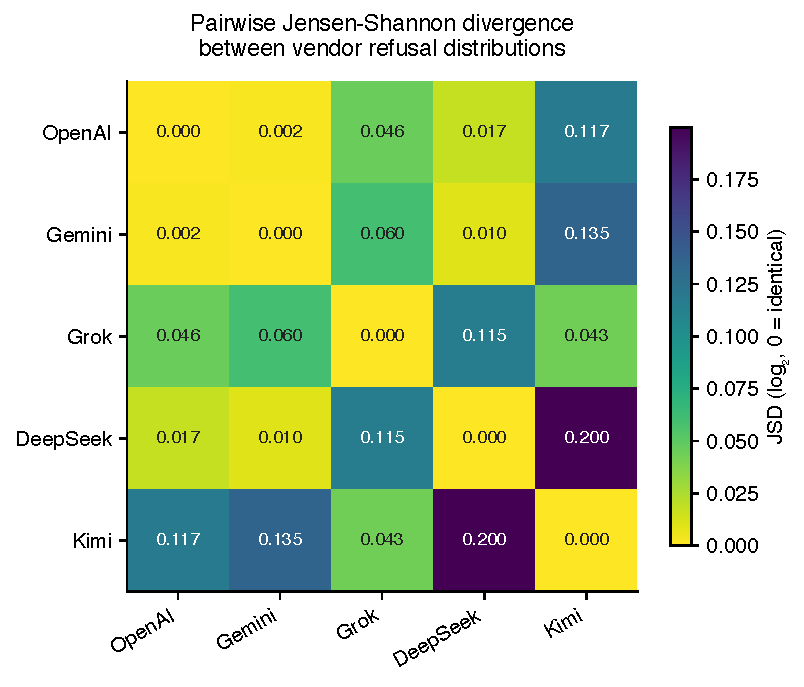
\includegraphics[width=0.7\textwidth]{fig2_pairwise_jsd_heatmap.pdf}
  \caption{Pairwise Jensen--Shannon divergence between vendors' 4-class
  refusal distributions (hard refusal, soft refusal, on-task, API-blocked).
  Values are base-2 bounded in $[0, 1]$. Diagonal is trivially zero.
  \vendor{DeepSeek} is near-minimal distance from both Western vendors
  (JSD $0.017$ from \vendor{OpenAI}, $0.010$ from \vendor{Gemini}) and
  maximally distant from \vendor{Kimi} (JSD $0.200$, the global maximum
  of the off-diagonal entries). \vendor{Kimi} is closest to \vendor{Grok}
  ($0.043$), not to its putative ``Chinese-vendor'' peer.}
  \label{fig:jsd-heatmap}
\end{figure}

Three features of this matrix together constitute the Finding~1 evidence.

\paragraph{(i) The Western baseline is statistically indistinguishable from zero.}
The \vendor{OpenAI}--\vendor{Gemini} JSD is $0.0019$ with 95\% bootstrap CI
\ci{0.0000}{0.0068}. Because this CI includes 0, the two distributions are
statistically indistinguishable at this sample size --- consistent with the
expectation that two U.S.\ RLHF pipelines trained with qualitatively
similar safety objectives produce qualitatively similar refusal patterns.

\paragraph{(ii) \vendor{DeepSeek} is close to the Western pair, not to \vendor{Kimi}.}
\vendor{DeepSeek}'s JSD to \vendor{OpenAI} is $0.017$ \ci{0.004}{0.034} and to
\vendor{Gemini} is $0.010$ \ci{0.001}{0.021}. Both intervals exclude zero
but only narrowly. In contrast, the \vendor{DeepSeek}--\vendor{Kimi} JSD
is $0.200$ \ci{0.149}{0.256} --- the largest value in the matrix and an
order of magnitude larger than either DeepSeek--Western comparison.

\paragraph{(iii) The CIs are mutually disjoint.}
The \vendor{DeepSeek}--\vendor{Kimi} 95\% CI (lower bound $0.149$) does not
overlap with \emph{any} CI involving \vendor{DeepSeek} and a Western vendor
(upper bound at most $0.034$). This non-overlap rules out the null
hypothesis that \vendor{DeepSeek} is equidistant from \vendor{Kimi} and
from the Western cluster at the 95\% confidence level.

\paragraph{Implication.}
These observations are inconsistent with a vendor-clustering axis organized
by national origin. The empirically supported partition is
$\{\vendor{OpenAI},\vendor{Gemini},\vendor{DeepSeek}\}$ against
$\{\vendor{Kimi}\}$, with $\vendor{Grok}$ occupying an intermediate position
(its closest neighbor is $\vendor{Kimi}$ at JSD $0.043$, driven by both
vendors' common pattern of high on-task rate; see §\ref{sec:results-finding3}).
We interpret this clustering structure as evidence that refusal-distribution
\emph{shape} (the relative mix of hard, soft, on-task, and API-blocked
categories) is dominated by RLHF training conventions rather than by
regulatory geography. DeepSeek, despite its Chinese corporate origin,
produces a refusal distribution whose shape closely tracks
contemporary U.S.\ RLHF practice. Kimi's distribution, by contrast, is
dominated by two vendor-specific departures: a non-zero API-level
content filter (7.0\% of calls; §\ref{sec:results-finding2}) and an
unusually high on-task rate (83.0\%) on the responses that pass the
filter. These two features together place Kimi far from every other
vendor in 4-class distribution space.

Section~\ref{sec:results-finding5} will further complicate this picture:
although DeepSeek's \emph{distribution shape} matches the Western cluster,
its \emph{topic-level behavior} diverges dramatically from both Western
vendors and from Kimi on sovereignty-adjacent prompts. The shape-level
similarity in Figure~\ref{fig:jsd-heatmap} thus masks a layer-specific
divergence that becomes visible only under per-topic stratification.

\subsection{Finding 2: Kimi's API Filter Is Taiwan-Statehood Blocking, Not Opinion Blocking}\label{sec:results-finding2}

\todo{Write in Batch 2. Lead with Fig 3 2-panel. Key evidence:
- 7.0\% of Kimi calls are API-level refusals, vs 0\% for all other vendors.
- By topic: sovereignty 23.1\%, factual 12.5\%, other topics 0\%.
- By expected: HR 11.2\%, OT 8.0\%, SR 1.4\%.
- All 14 blocked prompts in Appendix A. Critical subset: 4 OT-expected
  factual questions about RoC state institutions (legislature seats,
  constitutional amendments, presidential term, flag design) are blocked.
- Implication: filter triggers on institutional-recognition content,
  not on opinion elicitation. $\sim$0.8 page.}

\subsection{Finding 3: \vendor{Grok} and \vendor{Kimi} Share a Low-Refusal Regime via Different Mechanisms}\label{sec:results-finding3}

\todo{Write in Batch 2. Lead with Fig 4. Both 17\% refusal rate (CIs
\ci{12}{22}), 22.5pp below median. But Grok has 0\% api_blocked and
model-level permissive RLHF; Kimi has 7\% api_blocked with near-
100\% model-level on-task once past the filter. Different architectures,
similar aggregate. $\sim$0.5 page.}

\subsection{Finding 4: A Two-Layer Refusal Architecture}\label{sec:results-finding4}

\todo{Write in Batch 2. No standalone figure --- references Fig 3, Fig 4,
Fig 6. Frame as a conceptual summary: pre-generation infra filter (Layer 1,
only Kimi) + model-level RLHF (Layer 2, all vendors). Total observed
restrictiveness is a product, not sum. $\sim$0.5 page.}

\subsection{Finding 5: A 4-Profile Vendor Taxonomy via Topic-Stratified On-Task Rate}\label{sec:results-finding5}

\todo{Write in Batch 2. Lead with Fig 6 heatmap. This is the single
strongest signal in the dataset and the core §5 Discussion hook.

Key claim: DeepSeek sovereignty on-task = 10.3\% \ci{2.6}{23.3}, vs non-sov
54.0\%, gap -43.8pp. This CI is disjoint from every other vendor's
sovereignty CI. Contrast with Kimi sovereignty 83.3\% \ci{64.5}{93.8}
(topic-agnostic post-filter) and Grok 82.1\% \ci{65.9}{92.1}
(topic-agnostic no-filter).

Taxonomy (4 profiles):
  Profile A (Western: OpenAI, Gemini): moderate sovereign dampening
  Profile B (DeepSeek): topic-specific RLHF collapse
  Profile C (Grok): topic-agnostic permissive
  Profile D (Kimi): infra-filter + post-filter permissive

Paper's conceptual contribution: alignment culture is NOT a single axis.
Vendor behavior is a topic × vendor × layer 3-way interaction.

$\sim$1.0 page.}

\subsection{Finding 6: Prompt Bank Validity}\label{sec:results-finding6}

\todo{Write in Batch 2. Short section: OT baseline 96.4\% on-task validates
the prompt bank as producing the expected compliance distribution on
neutral factual questions. HR-expected producing 3\% hard / 55.8\% soft /
39.0\% on-task confirms RLHF engage-with-hedge over block. $\sim$0.3 page.}

\subsection{Finding 7: Two-Tier HR→SR Refusal Elasticity}\label{sec:results-finding7}

\todo{Write in Batch 2. Lead with Fig 5. OpenAI/Gemini +46pp Δ (responsive
RLHF) vs Grok/DeepSeek/Kimi +25--27pp Δ (clustered but for two reasons).
Clarify ceiling-effect (Grok/Kimi start high) vs stiff RLHF (DeepSeek
starts low, stays low). $\sim$0.5 page.}


\section{Discussion}\label{sec:discussion}
\todo{Write in Batch 2 after all §4 results are drafted.}

\section{Limitations}\label{sec:limitations}
\todo{Write in Batch 3. Key items:
(a) single-rater annotation with 24.5\% AI-advised (§3.5 discloses κ
infeasible, released audit trail);
(b) model-tier asymmetry (OpenAI/Gemini mini-class vs DeepSeek/Kimi flagship);
(c) single time-slice (April 2026 model IDs frozen);
(d) Taiwan-political domain only, findings may not generalize to other
politically-sensitive domains;
(e) N=200 prompts is modest for sub-topic claims (topic-level CIs wide).}

\section{Conclusion and Future Work}\label{sec:conclusion}
\todo{Write in Batch 3.}


% ── Bibliography ─────────────────────────────────────────────────────────
\printbibliography

% ── Appendix ─────────────────────────────────────────────────────────────
\appendix

\section{All Kimi API-Blocked Prompts ($N=14$)}\label{app:blocked}
\todo{Write in Batch 3. Include 14 prompts in original Chinese with English
glosses, grouped by expected category.}

\end{document}
